
%%True false commands %{
\newcommand{\T}{\textcolor{green!65!black}{\contour{black}{T}}}
\newcommand{\F}{\textcolor{red}{\contour{black}{F}}}
\newcommand{\uT}[2]{\only<#1-#2>{\T}}
\newcommand{\uF}[2]{\only<#1-#2>{\F}}
%}
\begin{frame}{}
    \textbf{Boolean Algebra:} Things are either true or false
    \begin{columns}[c]
        \begin{column}{.4\textwidth}
            % \vspace{-30pt}
            \only<-23>{%
            \begin{itemize}
                \item <2->"I am alive." ($A$)
                \item[] <6-> \hspace{.5cm}\only<6-19>{AND ($\wedge$)} \only<20->{\textbf{OR} ($\vee$)}
                \item <7-> "I am an elephant." ($E$)
            \end{itemize}
            \forestset{  
                	L1/.style={rectangle, rounded corners, shade, top color=white,     bottom color=blue!50!black!20, draw=blue!40!black!60, very     thick},   	
                	L2/.style={rectangle, rounded corners, shade, top color=white,     bottom color=blue!50!black!20, draw=blue!40!black!60, very     thick,
                		edge={black,line width=1.15pt,line cap=round,->}},   	
                	L3/.style={rectangle, rounded corners, shade, top color=white,     bottom color=blue!50!black!20, draw=blue!40!black!60, very     thick,
                		edge={black,line width=1.15pt,line cap=round,->}},   	
                	L4/.style={rectangle, rounded corners, shade, top color=white,     bottom color=blue!50!black!20, draw=blue!40!black!60, very     thick,
                	edge={black,line width=1.15pt,line cap=round,->}}, 
                }
            \uncover<3->{
                \begin{forest} 
            	for tree={
            		scale=.75,        
            		grow=0,
            		reversed, %tree direction         
            		parent anchor=east,
            		child anchor=west, %edge anchors   		edge={line cap=round},
            		outer sep=+1pt, %edge/node connection  		rounded corners,
            		minimum width=15mm,
            		minimum height=8mm, %node shape         l 		sep=10mm %level distance     
            		}   
                    [Start,L1,visible on=<3-> %%for children={visible on=<2->}%%
                    	[\T,L2, visible on=<4->         
                    		[\T,L3,visible on=<9->                     
                    		]         
                    		[\F,L3,visible on=<15->           
                    		]               
                    	]     
                    	[\F,L2,visible on=<5->         
                    		[\T,L3,visible on=<17->                     
                    		]         
                    		[\F,L3,visible on=<18->           
                    		]               
                    	] 
                    ] 
                \end{forest}
            }
        }
            \begin{figure}
                \centering
                \includegraphics<24->[width=.75\textwidth]{./images_5-20-2022/circuit0.png}
            \end{figure}
            \includegraphics<25->[width=.75\textwidth]{./images_5-20-2022/circuit1.png}
        \end{column}
        %%%%
        \begin{column}{.4\textwidth}
            \centering
            \only<8-21>{%
                \begin{tabular}{cc|c}
                     & \multicolumn{1}{c}{} & \tabularnewline
                     & \multicolumn{1}{c}{} & \tabularnewline
                    \textbf{$A$} & \textbf{$E$} & \textbf{$A\only<-20>{\wedge}\only<21>{\vee} E$}\tabularnewline
                    \hline 
                    \uT{8}{} & \uT{9}{} & \uT{10}{}\tabularnewline
                    \uT{15}{} & \uF{15}{} & \uF{16}{20}\uT{21}{}\tabularnewline
                    \uF{8}{} & \uT{17}{} & \uF{17}{20}\uT{21}{}\tabularnewline
                    \uF{18}{} & \uF{18}{} & \uF{19}{}\tabularnewline
                \end{tabular}} 
            \only<22->{
                \begin{tabular}{cc|c}
                     & \multicolumn{1}{c}{} & \tabularnewline
                     & \multicolumn{1}{c}{} & \tabularnewline
                    \textbf{$A$} & \textbf{$E$} & \textbf{$A \vee E$}\tabularnewline
                    \hline 
                    1 & 1 & 1 \tabularnewline
                    1 & 0 & 1 \tabularnewline
                    0 & 1 & 1 \tabularnewline
                    0 & 0 & 0 \tabularnewline
                \end{tabular}
            }
            \\ 
            % \vspace{10pt}
            %venn diagrams
            \begin{figure}
                \centering
            \includegraphics<11>[width=.75\textwidth]{./images_5-20-2022/venn_basic.pdf}
            \includegraphics<12>[width=.75\textwidth]{./images_5-20-2022/venn_A.pdf}
            \includegraphics<13,21>[width=.75\textwidth]{./images_5-20-2022/venn_A_or_B.pdf}
            \includegraphics<14-20>[width=.75\textwidth]{./images_5-20-2022/venn_A_and_B.pdf}
            \includegraphics<23->[width=1.25\textwidth]{./images_5-20-2022/ARM_binary.jpg}
            \end{figure}
        \end{column}
    \end{columns}
    
    \begin{tikzpicture}[remember picture, overlay]
        \node<26> [shift={(0,0)}] at (current page.center) { 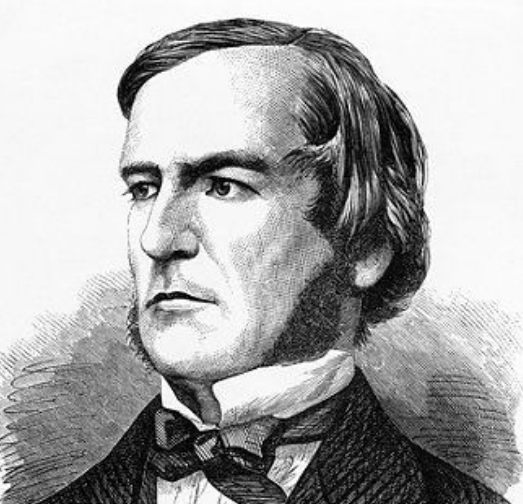
\includegraphics[scale=0.4]{./images_5-20-2022/Boole.png} };
        \node<27> [shift={(0,0)}] at (current page.center)
        { 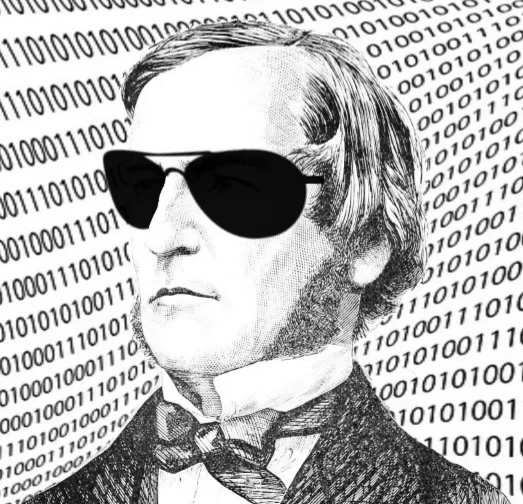
\includegraphics[scale=0.4]{./images_5-20-2022/BooleCool.png} };
    \end{tikzpicture}
\end{frame}

%%%recap-2%%%
\begin{frame}<9->{D420, D421, D422}
    \begin{columns}
        \begin{column}{.5\textwidth}
            \textbf{D420 \hl<7->{Discrete} Math-Logic}
            \begin{itemize}
                \item \hl<2->{Logic} \& \hl<3->{Proofs}
                \item \hl<9->{Boolean Algebra \& Boolean Functions}
            \end{itemize}
            %%
            \textbf{D421 \hl<7->{Discrete} Math-Functions \& Relations}
            \begin{itemize}
                \item \hl<5->{Set Theory}, \hl<6->{Finite Sequences, \& Series}
                \item \hl<6->{Relations} \& \hl<11->{Directed Graphs}
            \end{itemize}
            % %%
            \textbf{D422 \hl<7->{Discrete} Math-Functions \& Relations}
            \begin{itemize}
                \item \hl<7>{Algorithms}, linear \& associated Big-$\mathcal{O}$
                \item Number Theory \& Cryptography
            \end{itemize}
        \end{column}
        \begin{column}{.5\textwidth}
            \begin{figure}
                \centering
                \includegraphics<3>[width=.5\textwidth]{./images_5-20-2022/proofs.png}
                \includegraphics<4>[width=.5\textwidth]{./images_5-20-2022/proofs.png}
                \includegraphics<5>[width=.5\textwidth]{./images_5-20-2022/sets.png}
                \includegraphics<6>[width=.5\textwidth]{./images_5-20-2022/series.png}
                \includegraphics<7>[width=.65\textwidth]{./images_5-20-2022/discrete.png}
                \includegraphics<8>[width=.65\textwidth]{./images_5-20-2022/cont.png}
                \includegraphics<9>[width=.65\textwidth]{./images_5-20-2022/boolean.png}
                \includegraphics<10>[width=.65\textwidth]{./images_5-20-2022/binary.png}
                \includegraphics<11>[width=.65\textwidth]{./images_5-20-2022/graphs.png}
            \end{figure}
        \end{column}
    \end{columns}
\end{frame}

%%%%RSA alice and bob
\begin{frame}{} %alice and bob RSA
    \centering
    \adjustbox{max width =\textwidth, min height=8cm}{%
    \begin{tikzpicture}[scale=.8]
        % Include the image in a node
        \foreach \n  in {1,...,6}
            \node<\n> [above right,inner sep=0] at (0,0) {\includegraphics[]{./images_5-20-2022/alice_bob_RSA_\n.png}};
        \node<6>[font=\Huge] at (3.15,8.5) {\textbf{?}};
        
        \def\x{5.75}
        \def\y{7}
        \node<7-10> [above right,inner sep=0] at (0,0) {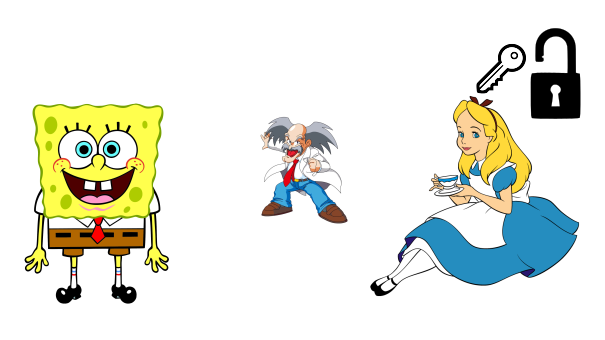
\includegraphics[]{./images_5-20-2022/alice_bob_RSA_7.png}};
            \node<8-10>[rectangle,draw,inner sep =5pt,align=center,font=\Large] at (10,9) {$c\equiv (\text{message})^{e}(\text{mod } N$)}; 
            \node<9-10> [font=\Large,draw, fill=white,align=center] at (10,2.75) {$N = p\times q$ for \textit{secret primes} $p$ \& $q$\\$e$ such that $\gcd(e,(p-1)(q-1)=1$};
            \node<10> [font=\Large,draw, fill=white] at (18.375,8.1) {$N$,$e$};
            
        \node<11-12> [above right,inner sep=0] at (0,0) {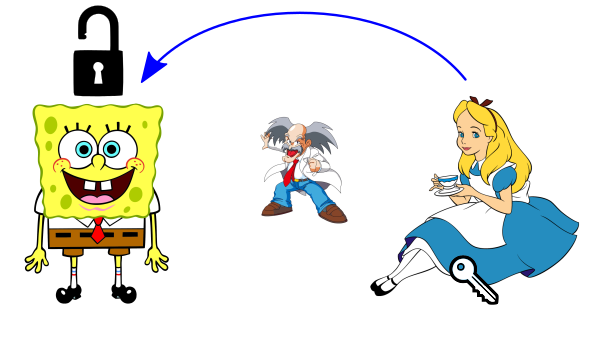
\includegraphics[]{./images_5-20-2022/alice_bob_RSA_9.png}};
            \node<11-12>[font=\Large,draw, fill=white] at (3.25,8.85) {$N$,$e$};
            \node<11-12>[font=\Large,draw, fill=white] at (15.5,2) {$p,q$};
            % \node<12> [font=\Large,right,draw, fill=white,align=center] (a) at (\x,2.75) {$e\times d \equiv 1(\text{mod} (p-1)(q-1))$};
    
    \node<13> [above right,inner sep=0] at (0,0) {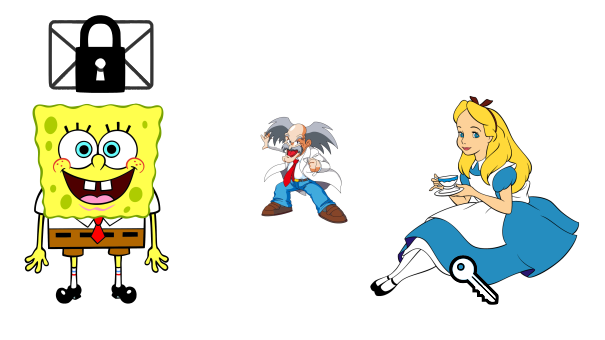
\includegraphics[]{./images_5-20-2022/alice_bob_RSA_10.png}};  
    \node<14> [above right,inner sep=0] at (0,0) {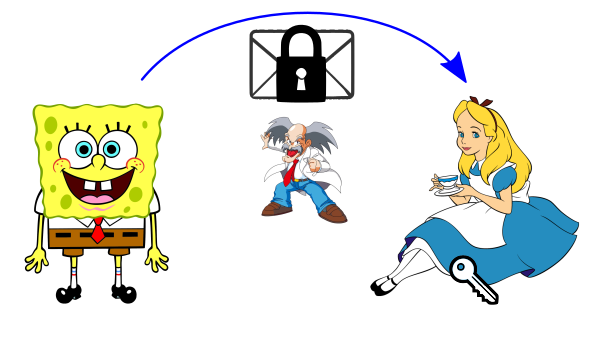
\includegraphics[]{./images_5-20-2022/alice_bob_RSA_11.png}};  
    \node<15> [above right,inner sep=0] at (0,0) {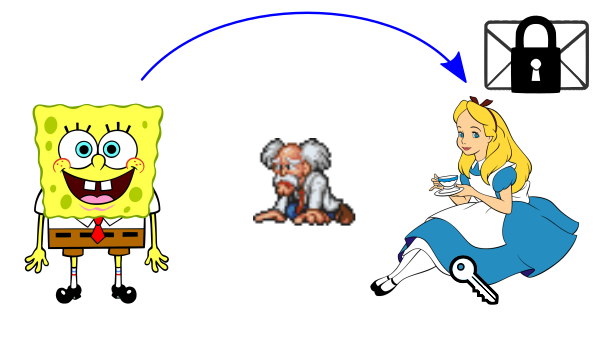
\includegraphics[]{./images_5-20-2022/alice_bob_RSA_12.png}};  
    \node<16-18> [above right,inner sep=0] at (0,0) {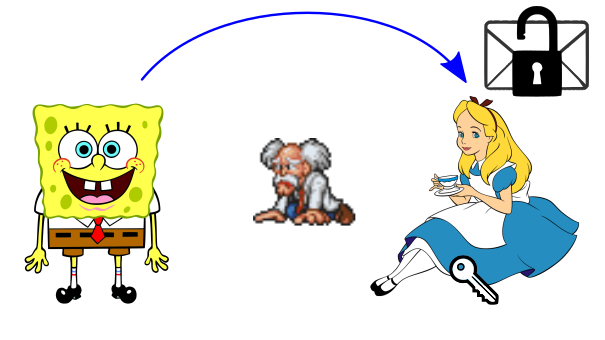
\includegraphics[]{./images_5-20-2022/alice_bob_RSA_13.png}};
        \node<17> [font=\Large,right,draw, fill=white,align=center] (a) at (\x,2.75) {$e\times d \equiv 1(\text{mod} (p-1)(q-1))$};
        \node<17>[font=\Large,draw, fill=white] at (15.5,2) {$p,q$};
        \node<18-19> [font=\Large,right,draw, fill=white,align=center] (a) at (\x,2.75) {$\text{message} \equiv c^{d}(\text{mod} N)$};
    
    \node<19-26> [above right,inner sep=0] at (0,0) {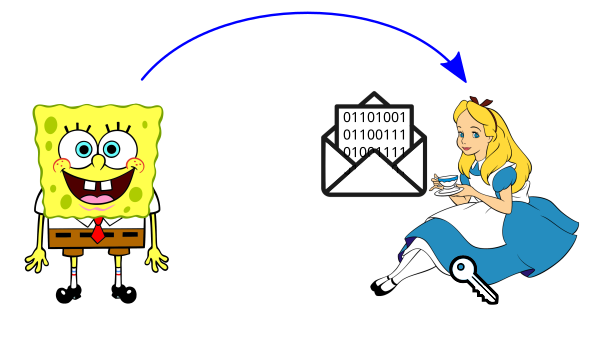
\includegraphics[]{./images_5-20-2022/alice_bob_RSA_14.png}};  
        \node<20-> [font=\Large,right] at (\x,\y) {$\bullet 01101001 \rightarrow$ \textbf{I}};
        \node<21-> [font=\Large,right] at (\x,\y-1) {$\bullet 01100111 \rightarrow$ \textbf{L}};
        \node<22-> [font=\Large,right] at (\x,\y-1.5) {$\bullet 01001111 \rightarrow$ \textbf{O}};
        \node<23-> [font=\Large,right] at (\x,\y-2) {$\bullet 01010110 \rightarrow$ \textbf{V}};
        \node<24-> [font=\Large,right] at (\x,\y-2.5) {$\bullet 01000101 \rightarrow$ \textbf{E}};
        \node<25-> [font=\Large,right] at (\x,\y-3.5) {$\bullet 01111001 \rightarrow$ \textbf{Y}};
        \node<26-> [font=\Large,right] at (\x,\y-4) {$\bullet 01001111 \rightarrow$ \textbf{O}};
        \node<27-> [font=\Large,right] at (\x,\y-4.5) {$\bullet 01010101 \rightarrow$ \textbf{U}};
    \node<27-> [above right,inner sep=0] at (0,0) {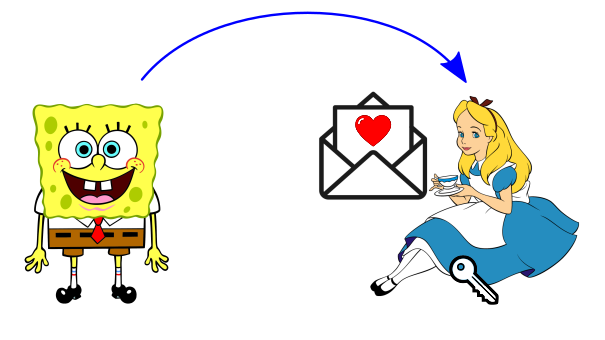
\includegraphics[]{./images_5-20-2022/alice_bob_RSA_15.png}}; 
    %guidelines
        % \draw[above right,help lines,step=1cm,gray!20] (0,0) grid (20,12);
    \end{tikzpicture}
    }
\end{frame}
%%%alice RSA time complexity
%{
\pgfplotsset{%
    axisA/.style = {%
        width=1.0\textwidth,
        % height=.5\textheight,
        % scale=1.0,
        axis lines=middle,
        xticklabels={,,}, yticklabels={,,},
        axis line style={-latex}, 
        ylabel={\footnotesize $f(n)$},             	
        xlabel={\footnotesize $n \rightarrow \infty$},
        x label style={at={(axis description cs:0.5,-0.05)},anchor=north},
        y label style={at={(axis description cs:-0.15,.5)},anchor=south},
        % clip=false, %doesn't clip outside graph
        domain=0:10,
        ymin=0,xmin=0,
        ymax=1000,xmax=25
    },
    axisB/.style = {%
        width=1.0\textwidth,
        % height=.5\textheight,
        % scale=1.0,
        axis lines=middle,
        xticklabels={,,}, yticklabels={,,},
        axis line style={-latex}, 
        ylabel={\footnotesize $f(n)$},             	
        xlabel={\footnotesize $n \rightarrow \infty$},
        x label style={at={(axis description cs:0.5,-0.05)},anchor=north},
        y label style={at={(axis description cs:-0.15,.5)},anchor=south},
        % clip=false, %doesn't clip outside graph
        domain=0:25,
        ymin=0,xmin=0,
        ymax=100,xmax=25
    }
}
\tikzset{
    plotA/.style = {thick, samples=50 
    %  domain=0:18.835
    },
    plotB/.style = {very thick, samples=50, dashed
    %  domain=0:18.835
    }
}
%} 

\begin{frame}{}
    \begin{columns}
        \begin{column}{.4\textwidth}
            \vspace{-6cm} \\
            \only<1-12>{%
                \only<6->{So how hard is it to factor?}
                \only<7->{$\approx 2^{(\text{number's length})}$ steps}
                \begin{itemize}
                    \item<8->[]$3\rightarrow 8$  
                    \item<9->[]$4\rightarrow 16$  
                    \item<10->[]$5\rightarrow 32$  
                    \item<11->[]$\dots$  
                    \item<12->[]$100\rightarrow 1.267\times 10^{30}$  
                \end{itemize}
            }
            \only<13->{%
                \begin{tikzpicture} 
                    \begin{axis}[axisA,plotA,ylabel={\footnotesize $2^{n}$},]
                    	\addplot[red]{2^x} node[above]{};
                    	\only<14>{%
                    	    \node (big-O) at (20,500) {\large \textcolor{red}{$\mathcal{O}(2^{n})$}};
                    	}
                    	\only<15->{%
                    	    \node (big-O) at (18,500) {\Huge \textcolor{red}{$\mathcal{O}(2^{n})$}};
                    	}
                    \end{axis}
                \end{tikzpicture}
            }
        \end{column}
        %%%%%%%%%%%%%%
        \begin{column}{.5\textwidth}
        \adjustbox{max width =\textwidth, min height=8cm}{%
            \begin{tikzpicture}[scale=.8]
            \node [above right,inner sep=0] at (0,0) {
\includegraphics[]{./images_5-20-2022/alice_RSA.png}};  
                \node<2> [font=\Large,draw, fill=white,align=center] at (5,10) {$N = p\times q$ for \textit{secret primes} $p$ \& $q$\\$e$ such that $\gcd(e,(p-1)(q-1)=1$};
                \node<3> [font=\huge,draw, fill=white,align=center] at (5,10) {$N$,$e$};
                \node<4> [font=\Large,draw, fill=white,align=center] at (5,10) {$e\times d \equiv 1(\text{mod} (p-1)(q-1))$};
                \node<5->[font=\huge,draw, fill=white,align=center] at (5,10) {$p,q$};
                % \draw[above right,help lines,step=1cm,gray!20] (0,0) grid (20,12);
        \end{tikzpicture}}
        \end{column}
    \end{columns}
\end{frame}